\documentclass[12pt, letterpaper]{memoir}
\usepackage{ExamStyle}

\begin{document}
	\pagestyle{empty}
	{\large Formulas}
	
	\begin{minipage}{0.5\linewidth}
		$q=mC\Delta T$
		
		$q=m\Delta H_{fus~or~vap}$
		
		 $\ln P_{vap} = \dfrac{-\Delta H_{vap}}{R}\left(\dfrac{1}{T}\right) + \ln\beta$	 
		
		$[Gas]=k_HP_{Gas}$
		
		$\Delta T_f = i \kappa_f m$
		
		$P_{A}=\chi_AP^\circ_A$
	\end{minipage}
	\begin{minipage}{0.5\linewidth}
		$q=nC\Delta T$
		
		$q=n\Delta H_{fus~or~vap}$
		
		$\ln\dfrac{P_2}{P_1}=\dfrac{-\Delta H_{vap}}{R}\left(\dfrac{1}{T_2} - \dfrac{1}{T_1}\right)$	
		
		$\Delta T_b = i \kappa_b m$
		
		$\Pi=\dfrac{nRT}{V}$
	
	\end{minipage}
	
	\vspace{2em}

	{\large Constants}
	
	$R=8.314 \dfrac{J}{mol~K}$
	
	$R=0.08206 \dfrac{L~atm}{mol~K}$
	

	
    \newgeometry{top=1mm, bottom=1mm, left=1mm, right=1mm}


\hspace{6em}	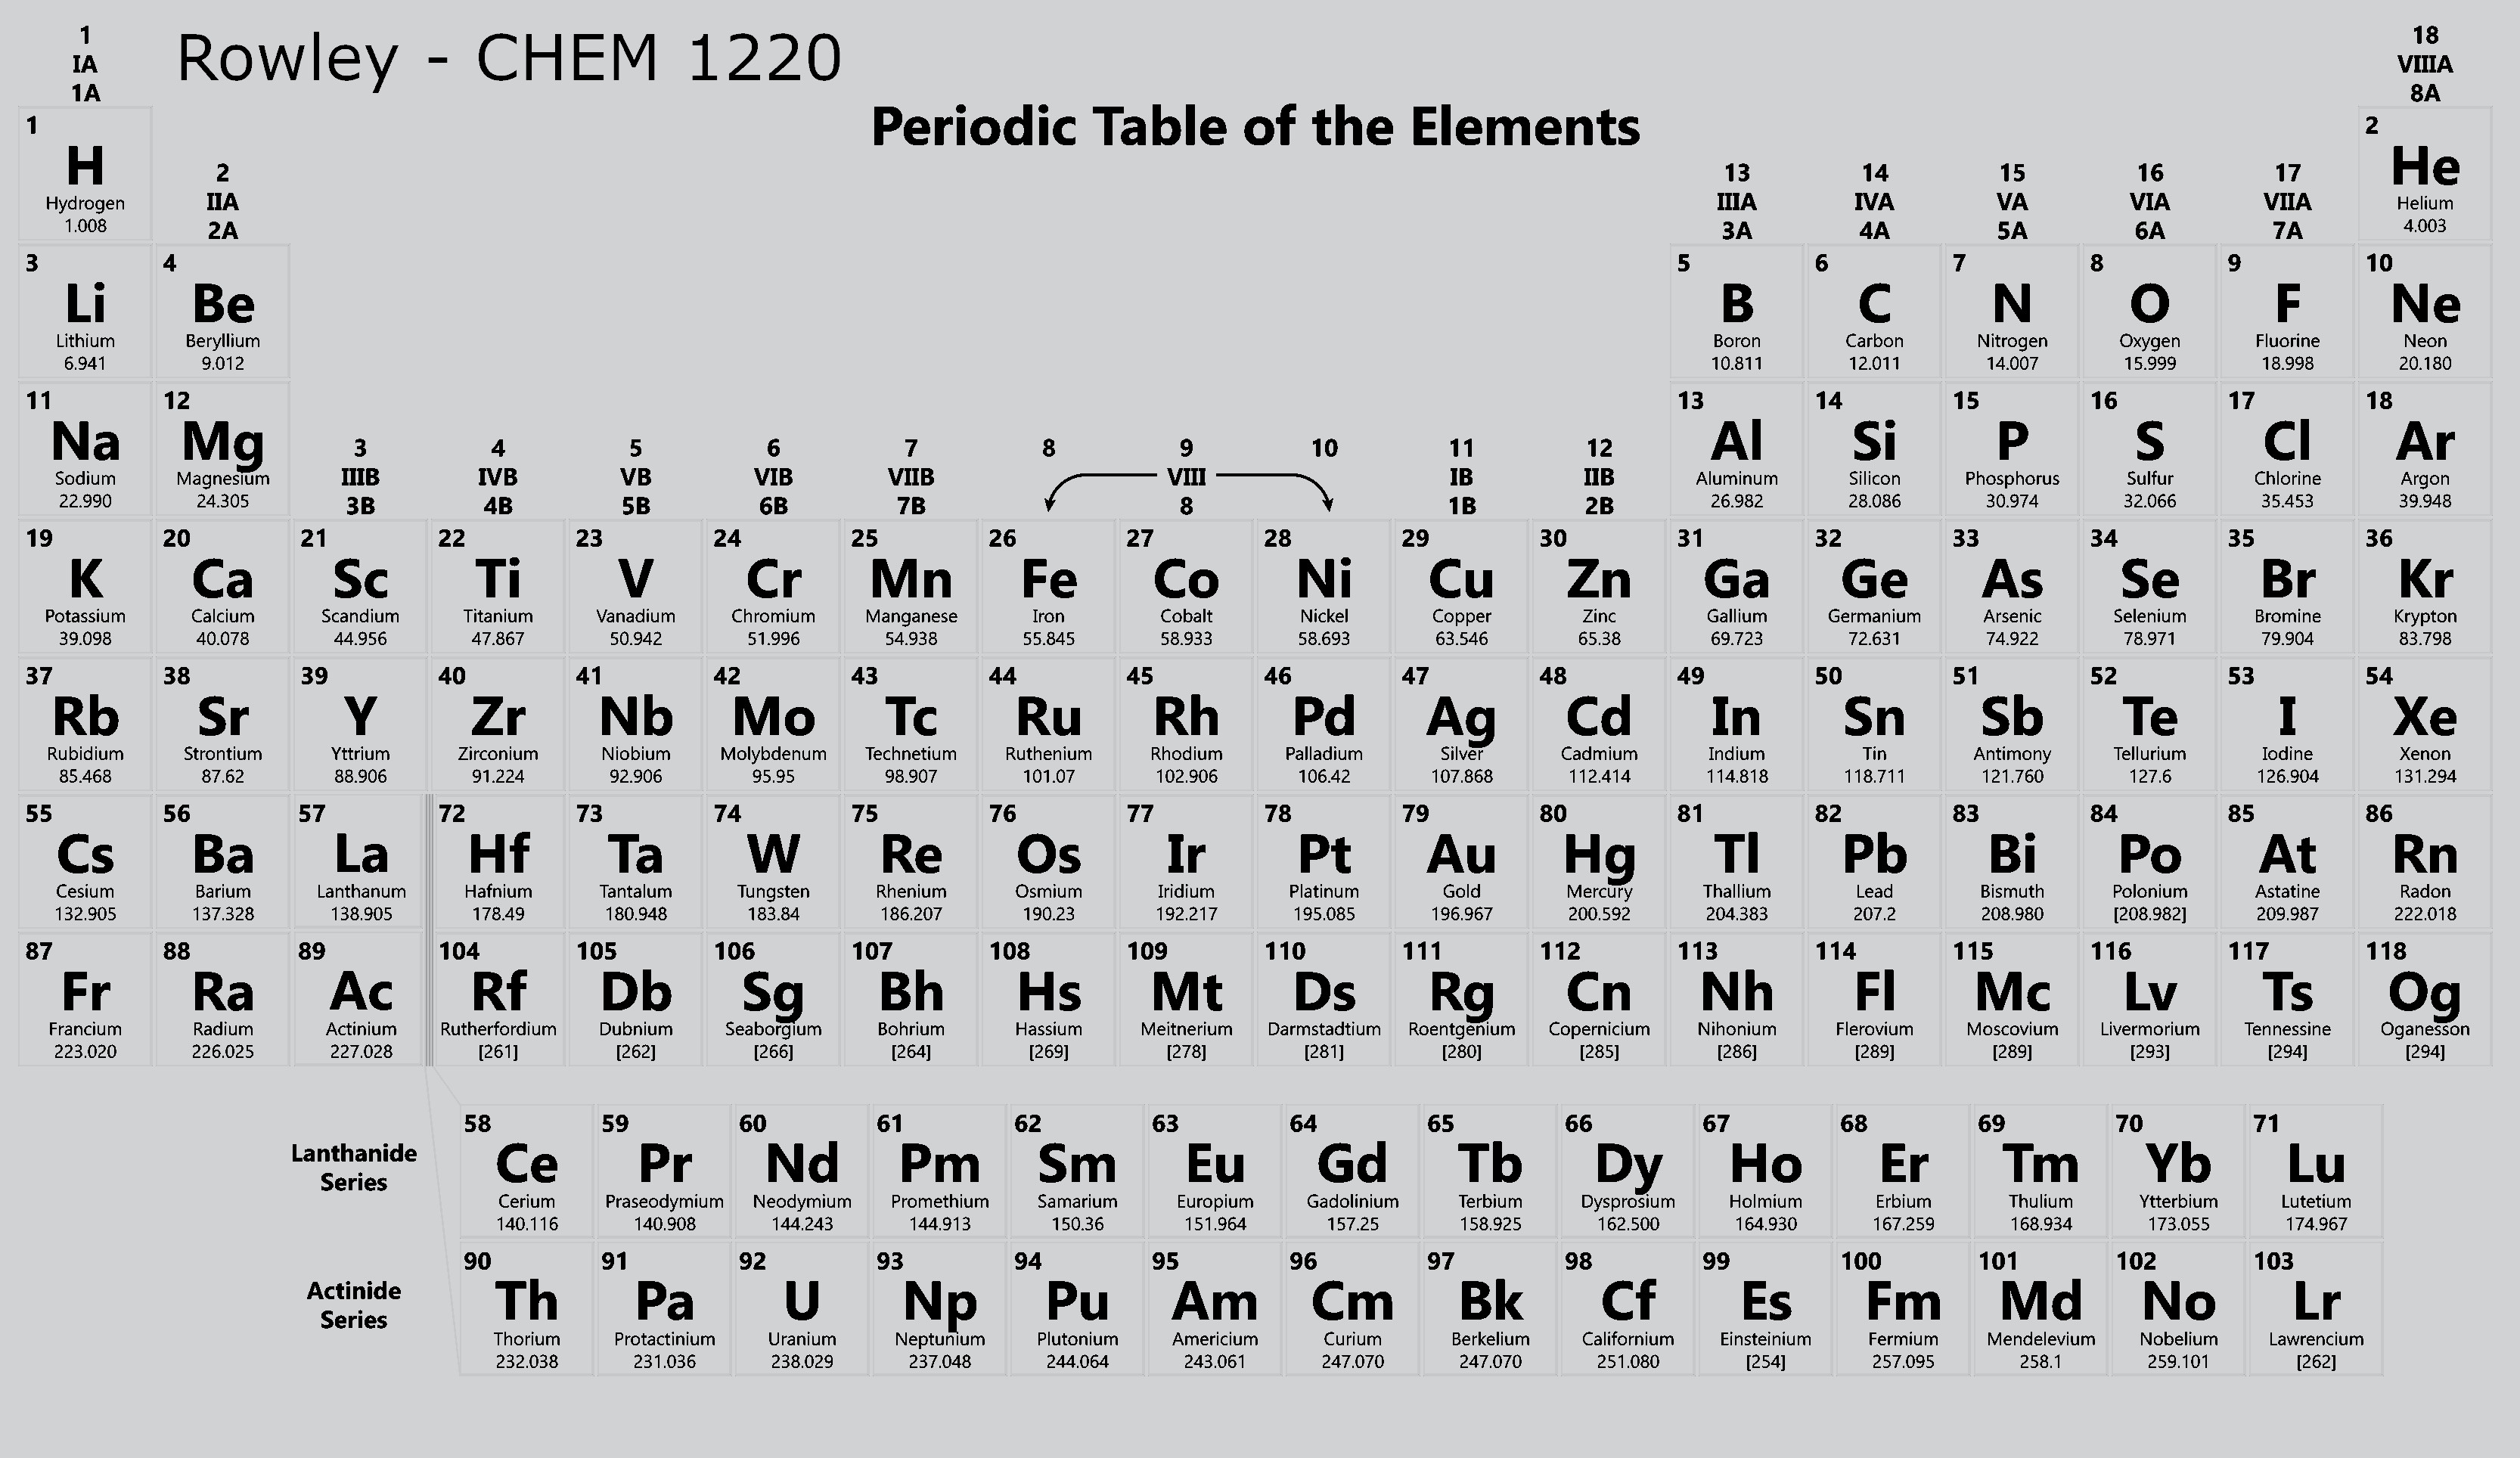
\includegraphics[width=1.3\textwidth, angle =90]{UpdatedTable}

	\restoregeometry

	
\end{document}